%!TEX root = ../paper.tex
\subsection{Discussions}
\label{sec:energy}

In this section we discuss (a) the energy implications of changing the clock speed, and (2) a possible Web page optimization for low-end devices based on our observations in \S\ref{label:web}.

%\begin{figure}[t]
%  \centering
%  \subfloat[Youtube and Skype]{
%  \includegraphics[width=0.9\linewidth]{sections/power-video}}
%  
%\subfloat[Web page load]{
%  \includegraphics[width=0.9\linewidth]{sections/power-plt}
%  }
%  \caption{Energy consumption vs. clock rate for
%  (a) video streaming and telephony and (b) Web page load}
%   %\vspace{-0.15in}
%\label{fig:power-video-web}
%\end{figure}

\begin{figure*}
    \begin{subfigure}[b]{0.5\textwidth}
        \centering
        \includegraphics[width=1\linewidth]{sections/device-work/power-video}
    	 \caption{\textit{Youtube and Skype}}
    \end{subfigure}
    \begin{subfigure}[b]{0.5\textwidth}
        \centering
        \includegraphics[width=1\linewidth]{sections/device-work/power-plt}
   	\caption{\textit{Web page load}}
    \end{subfigure}
  \caption{Energy consumption vs. clock rate for (a) video streaming and telephony and (b) Web page load}
  \label{fig:power-video-web}
  \vspace{-0.15in}
\end{figure*}

\subsubsection{Energy Consumption}
CPU clock frequency has an impact on the device's energy consumption and here low end devices may win. To evaluate 
energy consumption we use the same set up as the one described in \S\ref{sec:setup}. The experiments are conducted on the Nexus 4 phone and we use the Snapdragon Profiler~\cite{qualsnap} to log the energy consumption. The profiler samples energy at a high sampling rate of 20 times a second. %energy consumption \todo{do we know anything about the accuracy of the profiler?}. \mallesh{The profiler has different sampling rates (50ms, 120ms, 240ms) at which the metrics can be collected. We use minimum value 50ms.}

Figure~\ref{fig:power-video-web}
shows the energy consumption for all three applications
considered in this study with increasing 
clock frequency. Figure~\ref{fig:power-video-web}(a) shows the energy consumption while running YouTube and Skype at different frequencies. With increase in CPU clock frequency energy consumption increases steadily - somewhat faster for telephony (Skype) than streaming (YouTube). One reason for this is that YouTube prefetches video content. This allows the network to be inactive after the required content is prefetched. But Skype is interactive requiring that the network remain active throughout the session. 

Overall, the energy consumptions are more
drastic than the QoE improvements in these two applications
with faster clocks. For example, from the slowest end to fastest
end of clock frequency 1) Skype consumes $7\times$ more 
energy  while providing about $2\times$ better
frame rate; 2)  YouTube provides a modest
improvement of startup latency, $\approx$1 sec vs. 
$\approx$3 sec for about a 5 min video, but consumes
$5\times$ more energy. 

For Web page load (Figure~\ref{fig:power-video-web}(b)), 
the observation is different. As CPU frequency increases, the 
energy consumption first decreases and then increases. This 
is because initially the faster page load compensates
more than the increased power draw due to faster 
clock. Recall that 
energy consumption = avg. power draw $\times$ time. Similar to the video example, energy consumption is more drastic than QoE improvement (Figure~\ref{fig:plt_clock}). % When the CPU speeds increases from 702 MHz to 1512 MHz, energy consumption increases by $3\times$ but the average PLT only decreases by 50\% by 

Thus, an optimal frequency exists if one is interested
in optimizing the energy consumption for applications. Currently, when the frequency governor~\cite{ad-governors} is set to power-saving, the application is set to use the lowest CPU frequency. Instead, one can design a governor that takes into account the marginal performance improvement and the resulting energy consumption. 

